\documentclass[a4paper,11pt]{article}

\usepackage[left=2cm, top=3cm, text={17cm, 24cm}]{geometry}
\usepackage[czech]{babel}
\usepackage[utf8]{inputenc}
\usepackage{times}
\usepackage[unicode]{hyperref}
\usepackage{amsmath}
\usepackage{graphicx}
\usepackage[margin=0.5cm]{caption}
\graphicspath{ {./img/} }
\hypersetup{hypertexnames = false}

\begin{document}
	\begin{titlepage}
		\begin{center}
			\textsc{\Huge Vysoké učení technické v~Brně\\
				\vspace{0.4em}\huge Fakulta informačních technologií}
			
			\vspace{\stretch{0.382}}
			
			{\LARGE Modelování a simulace\\
				\Huge Predikce epidemie COVID-19\\ \vspace{0.3em}}
			
			\vspace{\stretch{0.618}}
			
			{\Large \hfill Radek Švec (xsvecr01)\\ \today \hfill Martin Kostelník (xkoste12)}
		\end{center}
	\end{titlepage}

	\section{Úvod}
		Tématem práce jsou epidemiologické modely na makroúrovni, konkrétně předpovídání šíření pandemie COVID-19 na území Itálie a České republiky. Tato práce implementuje již existující model vytvořený Giuliou Giordanem a dalšími \cite{source}, který předpovídá vývoj pandemie na území Itálie a opakuje provedené experimenty. Smyslem projektu bude předpovědět šíření nemoci COVID-19 na území České republiky v následujících měsících, vzít v úvahu různá opatření proti šíření a zhodnotit, zda byly dosavadně zavedené opatření dostačující, případně zda bylo rozvolnění těcho opatření správným rozhodnutím.
		
	\subsection{Autoři a zdroje informací}
		Autory tohoto projektu jsou:
		\begin{itemize}
			\item Radek Švec, xsvecr01@stud.fit.vutbr.cz
			\item Martin Kostelník, xkoste12@stud.fit.vutbr.cz
		\end{itemize}
	
	Jak bylo řečeno v úvodu, samotný model byl převzat z odborné literatury \cite{source}. Při pokusu aplikovat model na prostředí České republiky byly použity data z TODO ASI MZCR.
			
	\section{Popis abstraktího modelu}
		Model zvaný SIDARTHE je rozšířením jednoduššího SIR modelu, který rozděluje populaci na tři skupiny lidí (náchylné, infikované a vyléčené) o dalších pět skupin. Vzniká nám tedy následujících osm skupin.
		
		\begin{itemize}
			\item S -- Náchylní (Susceptible) k onemocnění.
			\item I -- Nakažení (Infected), kteří jsou asymptotyčtí a nedetekováni.
			\item D -- Diagnostikovaní (Diagnosed), kteří jsou asymptomatiční, avšak vir u nich byl detekován.
			\item A -- Nemocní (Ailing), kteří jsou symptomatiční, ale nebyli testovaní.
			\item R -- Léčící se (Recognized), kteří mají symptomy i u nich byl vir detekován.
			\item T -- Životně ohrožení (Threatened), kteří mají těžký průběh a je u nich vyžadována intenzivní péče.
			\item H -- Vyléčení (Healed).
			\item E -- Mrtví (Extinct).
		\end{itemize}
	
		\begin{figure}[h]
			\caption{Grafické znázornění modelu}
			\label{fig1}
			\centering
			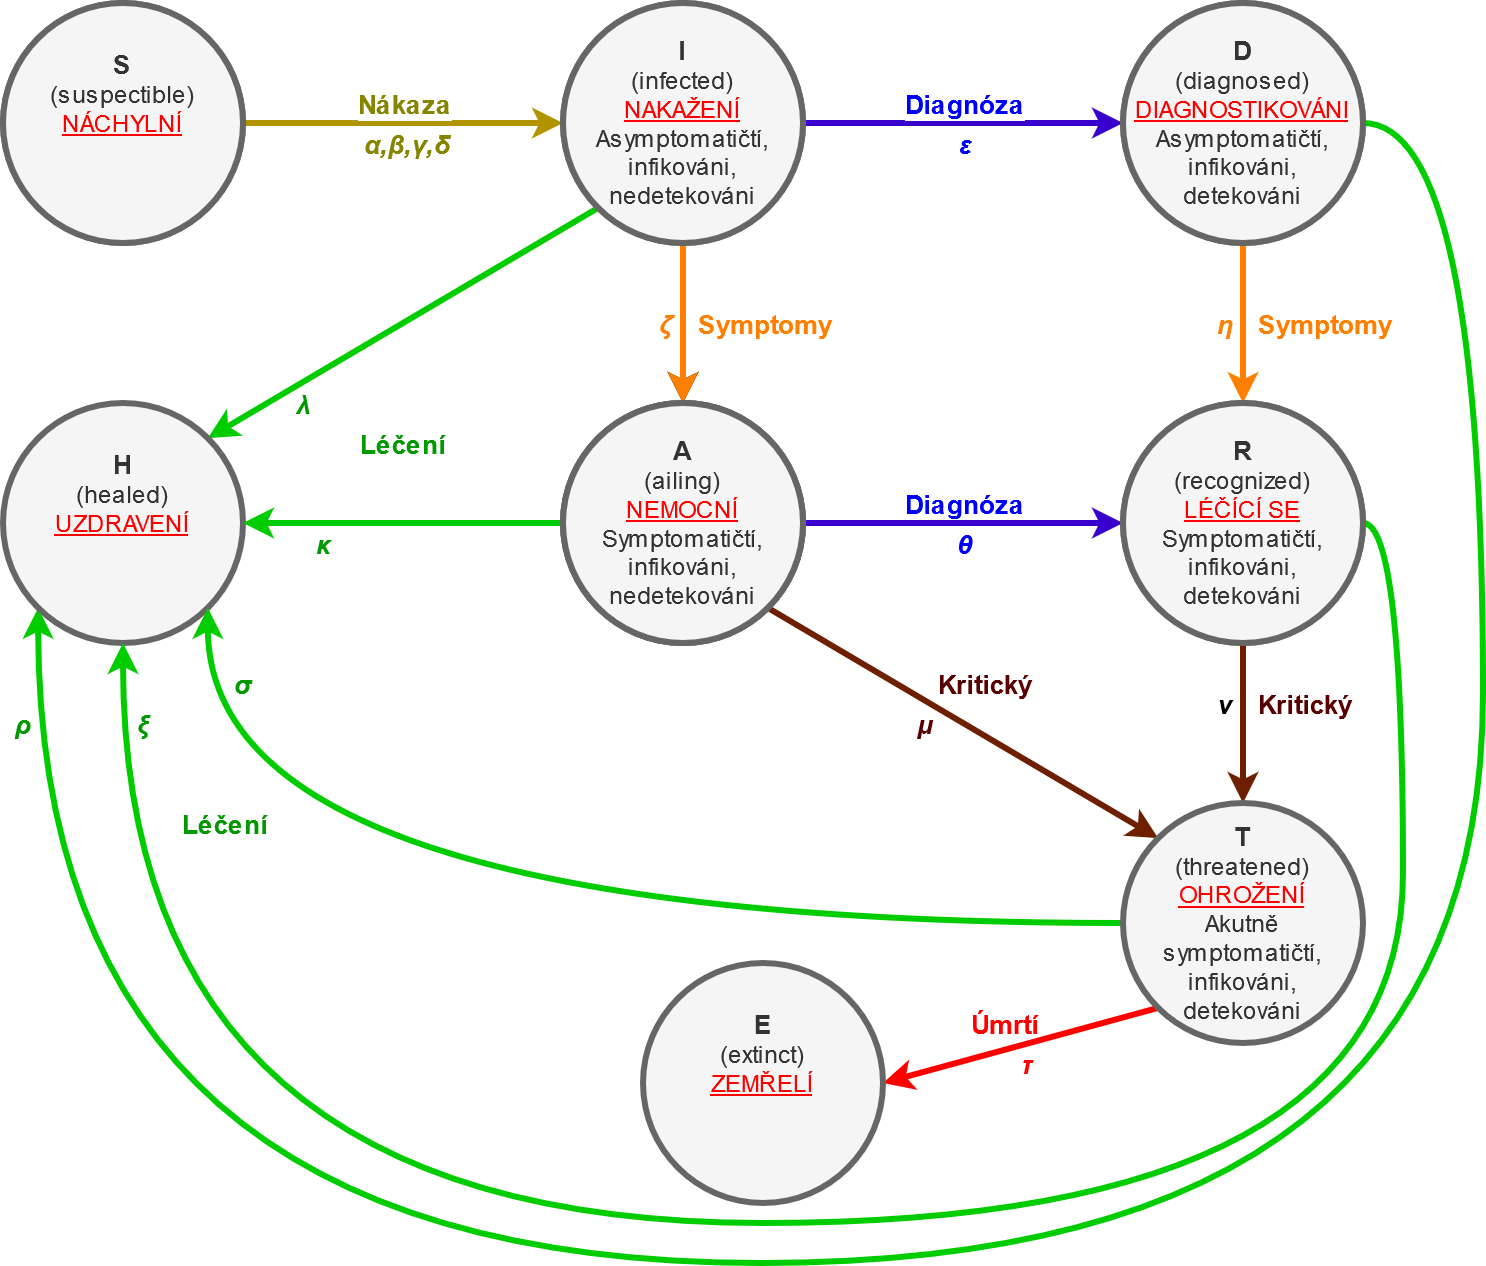
\includegraphics[scale=0.25]{model.png}
		\end{figure}
		\newpage
	
		Tento model nepočítá s možností, že se jedinec může virem nakazit opakovaně. Ikdyž bylo prokázáno, že se jedinec znovu nakazit může TADY OCITOVAT, není stále přesně známo, jakou imunitu si jedinec vybuduje. Takto nakažených je navíc velice malé množštví TADY DÁT ČÍSLO A OCITOVAT, tudíž je v modelu zanedbáváme.
		
		Model můžeme matematicky popsat celkem osmi diferenciálními rovnicemi, které popisují vývoj jedinců v každé skupině jako zlomek celkové populace státu.
		
		\begin{align}
			S'(t) &= - S(t) (\alpha I(t) + \beta D(t) + \gamma A(t) + \delta R(t))\\
			I'(t) &= S(t) (\alpha I(t) + \beta D(t) + \gamma A(t) + \delta R(t)) - (\epsilon + \zeta + \lambda)I(t)\\
			D'(t) &= \epsilon I(t) - (\eta + \rho) D(t)\\
			A'(t) &= \zeta I(t) - (\theta + \mu + \kappa) A(t)\\
			R'(t) &= \eta D(t) + \theta A(t) - (\nu + \xi) R(t)\\
			T'(t) &= \mu A(t) + \nu R(t) - (\sigma + \tau) T(t)\\
			H'(t) &= \lambda I(t) + \rho D(t) + \kappa A(t) + \xi R(t) + \sigma T(t)\\
			E'(t) &= \tau T(t)
		\end{align}
	
	Kromě velikostí jednotlivých skupin, se v rovnicích vyskytují následující paramtry:
	\begin{itemize}
		\item $\alpha$, $\beta$, $\gamma$, $\delta$ představují pravděpodobnost přenosu viru mezi náchylným jedincem a jedincem infikovaným, diagnostikovaným, nemocným a léčícím se v tomto pořadí vynásobenou průměrným počtem kontaktů za den.
		\item $\epsilon$, $\theta$ představují pravděpodobnost detekce viru u nakažených a nemocných.
		\item $\zeta$, $\eta$ -- představují pravděpodobnost, že se u nakaženého a diagnostikovaného jedince vystkytnou symptomy nemoci.
		\item $\mu$, $\nu$ představují pravděpodobnost, že se z nemocného a léčícího se jedince stane kriticky ohrožený jedinec.
		\item $\tau$ představuje úmrtnost.
		\item $\lambda$, $\kappa$, $\xi$, $\rho$ a $\sigma$ představují pravdepodobnost, že se nakažený, nemocný, léčící se, diagnostikovaný, nebo ohrožený jedinec z nemoci vyléčí.
	\end{itemize}
		
	\section{Implementace simulačního modelu}
	\section{Zopakování experimentů}
		V článku byly prováděny
	\section{Aplikování modelu na Českou republiku}
	\subsection{Experimenty}
			
	\section{Závěr}
		asdfasdfasdfasdfasdfasdfasdfasdfasdfasdfasdfasdfasdf
		asdfasdfasdfasdfasdfasdfasdfasdf

	\newpage
	\bibliographystyle{czechiso}
	\renewcommand{\refname}{Literatura}
	\bibliography{doc}
\end{document}